
\section{Social Graph}

In social graph mining, we often want to extract significant communities of users.

\subsection{Community evaluation}

Before extracting communities from a social graph, we need to define what is a strong community (well defined) and what is a weak communities (weak bounds between members).

\subsubsection{Strong or weak community}

For a given vertex $i$ we define
\begin{itemize}
  \item the internal degree $k_i^{int}$ the number of edges from $i$ going to another vertex of the community
  \item the external degree $k_i^{ext}$ the number of edges from $i$ going to a vertex outside of the community
\end{itemize}

For a node $i$ correctly assigned to a community $C$, we should have a high $k_i^{int}$ and a low $k_i^{ext}$. More formally

\[
  \sum_{i\in C} k_i^{int}(C) > \sum_{i\in C} k_i^{out}(C)
\]

\subsubsection{Modularity}

Modularity measures how well a graph $G$ is partitioned into communities $S$

\paragraph{Modularity.}
  \[
    Q \propto \sum_{s \in S} (\text{\# edges within } s) - (expected \text{ \# edges within } s)
  \]
  The expected value is computed on a graph with same degree distribution but random connections (null model).


\paragraph{Normalized modularity.}
  \[
    Q(G,S) = \underbrace{\frac 1 {2m}}_{\text{normalize}} \sum_{s\in S, i,j\in s} \l(A_{ij} - \frac{k_ik_j}{2m}\r)
  \]
  and $-1<Q<1$


Modularity is positive if the intra connection exceeds the expected number. A partitioning is significant if $Q>0.3,0.7$. We can use modularity to know when to stop community extraction algorithm (pick).

\subsection{Community extraction}

% We build a similarity matrix ($A_{ij}$ how node $i$ and $j$ are similar) from the adjacency matrix.

Hierarchical clustering algorithms identifies groups of nodes with high similarity. We can distinguish two strategies:

\begin{itemize}
  \item \textbf{Agglomerative algorithm:} merge nodes and communities with high similarity
  \item \textbf{Divisive algorithm:} split communities by removing links connecting nodes with low similarity (smallest cut)
\end{itemize}

In both strategy, we need a stopping point for the iterative process. Either we chose an arbitrary number of communities $k$ or we use a criteria (see modularity).

\paragraph{Girvan-Newman method.} Divisive hierarchical clustering based on edge betweenness. Iteratively remove edge of highest betweenness. Runs in $O(ln^2)$, $O(n^3)$ for sparse graph.

\paragraph{Louvain Modularity.} Greedy optimization in $O(n\log n)$, find small communities locally and then group smallest communities as simple nodes.

\subsubsection{Edge betweenness}

\paragraph{Edge betweenness.}
  Number of shortest paths passing over an edge (max $n(n-1)$)


\paragraph{Random walk betweenness.}
  Given two nodes $i$ and $j$, $x_{ij}$ is the probability that the edge between $i$ and $j$ is taken by a walk averaged over all the random walks between the pairs of node of the graph.


\subsubsection{How to compute betweenness ?} 

Repeat for each node, but let take $A$ w.l.o.g. (see \cref{fig:betweenness})

\begin{itemize}
  \item BFS from node $A$, all nodes are layered
  \item For each node $i$, count the number of shortest paths arriving to $i$. Recursively sum up the count of the parents (assigning 1 to node $A$).
  \item Assign edge values bottom up, each node has value $1 + \sum ($child edges weight$)$, to distribute proportionally to its parents according to their weight
  \item Repeat for each node, sum the weights and divide by two (paths discovered twice - from each end).
\end{itemize}


\begin{figure}
  \centering
  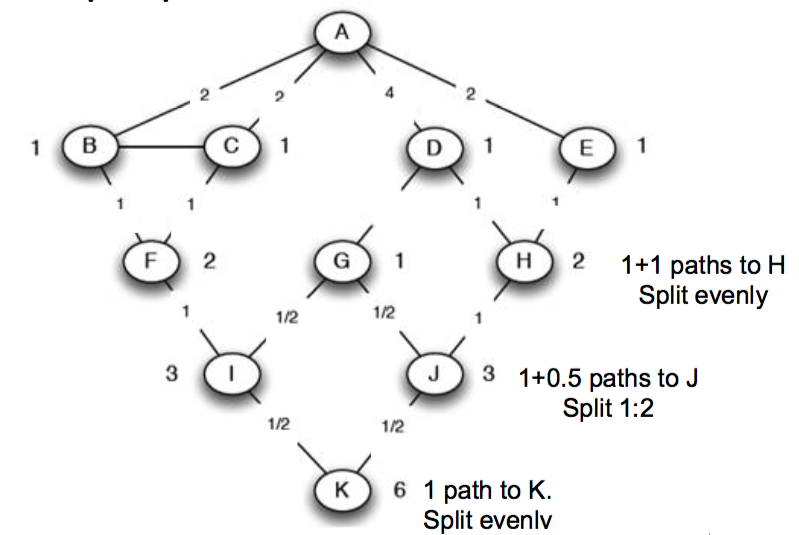
\includegraphics[width=1\linewidth]{figures/betweenness_computation.png}
  \caption{Betweenness computation - BFS, top down node weighting, bottom up edge values}
  \label{fig:betweenness}
\end{figure}

\subsubsection{$k$-medoids for cluster extraction}

We can use $k$-medoids with arbitrary chosen starting centers and a given distance function (weight on the edges for instance). Should start with multiple starting point to avoid being stuck in bad local optimum.

\subsection{Random graphs}

\paragraph{Small world graphs.}
  Graph for which most nodes are not neighbors of one another but most nodes can be reached from any other node by a small number of hops


\paragraph{Milgram's experiment.} Send a message from Nebraska to Massachusetts, from people to friends/relatives (mean of 5-6 hopes)

The experiment rises two problem, how to explain that there exists such short paths in  the social graph, and how to actually find these shortest paths efficiently ?

\subsubsection{Random graph model $G(n,p)$}

Simplest model, take $n$ nodes, connect each pair of nodes with probability $p$. It has the following properties

\begin{itemize}
  \item \textbf{low diameter}, expected distance between two nodes is $\log_k n$ with $k$ the average out degree,
  \item a pair $(i,j) \in V^2$ picked uniformly at random is connected by a short path with high probability
  \item \textbf{low clustering} coefficient (inaccurate for social graph modeling)
\end{itemize}

\paragraph{Diameter.}
  The diameter of a graph $G$ is the longest shortest path between any pair of nodes.

\paragraph{Local clustering coefficient.}
  The local clustering coefficient is the proportion of neighbors connected for a given node. Formally for a given node $i$ with neighbors $N$ and edges between them $E$
  \[
    C_i = \frac { 2|E|}{|N|(|N|-1)}
  \]

\paragraph{Global clustering coefficient.}
  Average of the local clustering coefficient.
  \[
    C = \frac 1 n \sum_i^n C_i
  \]

\subsubsection{Watts and Strogatz model}

Random rewiring of regular graph: take a regular graph and with probability $p$ rewire each link to a randomly selected node. Resulting graph has properties, both of regular and random graphs, see \cref{fig:watts_strogatz}.

\begin{figure}
  \centering
  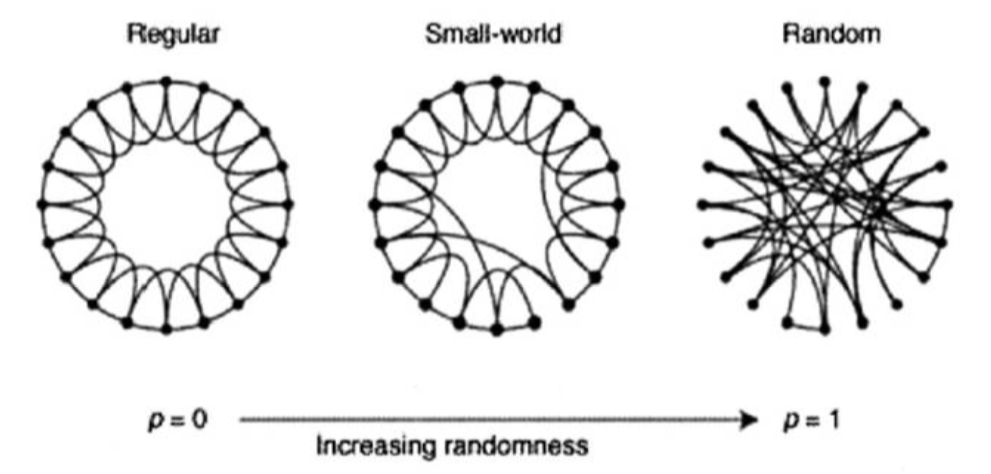
\includegraphics[width=1\linewidth]{figures/watts_strogatz_graph.png}
  \caption{Watts Strogatz rewiring construction}
  \label{fig:watts_strogatz}
\end{figure}

\subsubsection{Efficient search algorithm (Kleinberg’s model)}

\begin{itemize}
  \item Embed a graph into an $d$-dimensional grid to define a distance function ($l$2 norm for instance)
  \item each node is connected to $p$ of its closest neighbor (short range links) + $q$ random nodes (long range links) according to a distribution
  \[
    \P{u \leftrightarrow v} \propto \text{dist}(u,v)^{-r}
  \]
\end{itemize}

Decentralized routing algorithm performs well if and only if $r=$ dimension of the space. If $r$ is too small, we go far but struggle to converge, if $r$ is too high we stay among our neighbors, hard to reach the neighborhood of the target.

For $r=0$ we chose the long range links uniformly, like a random graph. there exist short paths between every pair of vertex but there is no decentralized algorithm capable of finding these paths efficiently.

\paragraph{Routing cost.} With $O(1)$ long range link $O(\log^2 n)$, and with $O(\log n)$ long range links $O(\log n)$.
